% !TeX root = bericht.tex
\section{Aufgabe 2: Behälter mit Wasserablauf}
Um den Sollwert stationär genau regeln zu können, wird im Folgenden ein Behälter mit Abfluss betrachtet. Der Abfluss $q_{ab}(t)$ in $[\frac{m^3}{s}]$ ist für den Regelkreis eine Störung. Im Modell wird diese nach der Regelstrecke abgezweigt und vor die Regelstrecke rückgekoppelt. Die Störung beeinflusst die Regelgröße $h$. Der Regelkreis muss mit einer Änderung des Zuflusses reagieren, um die Abweichung auszugleichen. 

\subsection{Linearisiertes Ausflussgesetz mit P-Regler}
Das erste Modell geht vereinfachend davon aus, dass der Abfluss proportional zur Füllhöhe ist. Der mathematische Zusammenhang ist in Gleichung (5) dargestellt.

\begin{equation}
    q_{ab}(t)= c \cdot h(t), \quad c=3\frac{l}{sm}
\end{equation}

Für dieses Modell wird das Modell in Abbildung \ref{blockschaltbild} um das Signal $q_{ab}$ erweitert, welches vor die Regelstrecke rückgekoppelt wird. Der effektive Zufluss $q_{eff}$ berücksichtig nun, dass das Wasser direkt wieder abfliesst. Vor der Regelstrecke wird $q_{eff}$ wie in Gleichung (6) berechnet.

\begin{equation}
    q_{eff}=q_{zu}-q_{ab}
\end{equation}

Der Regelkreis ist nicht stationär genau. Die Regelgröße nähert sich der Führungsgröße an. Die Stellgröße wird solange kleiner und die Störgröße größer, bis gilt: $q_{zu} = q_{ab}$. In diesem Fall ist der effektive Zufluss Null. Da aber der effektive Zufluss das Eingangssignal der Regelstrecke ist, wird die gesamte Regelstrecke zu Null gesetzt. Auch die Rückkopplung und damit die Regeldifferenz liefern nun den Wert Null. Aus Sicht des Regles heißt eine Regeldifferenz von Null, dass die Regelgröße gleich der Führungsgröße ist. Damit ist die Regelung abgeschlossen, obwohl der gewünschte Füllstand noch nicht erreicht wurde. Der tatsächliche Füllstand heißt stationärer Endwert. Die Differenz zwischen der gewünschten Sollhöhe und dem stationären Endwert nennt man die absolute Regelabweichung. Je größer die Reglerverstärkung $K_r$ wird, desto kleiner wird die Abweichung. Eine vollständige Kompensation ist nur theoretisch möglich für $K_r \to \infty$. Praktisch ist ein P-Regler nicht geeignet für diese Aufgabe. Deswegen wird der P-Regler später durch einen integralen Anteil erweitert werden.

Der Regelkreis wurde mit den selben fünf Reglerverstärkungen wie in Aufgabe 1 modelliert. Der Code ist in \ref{code_2a} dargestellt. Abbildung \ref{blockschaltbild_a} zeigt das Blockschaltbild des Regelkreises. Abbildung \ref{fig:a_plots_mit_abfluss} zeigt die zeitlichen Verläufe der Signale für die verschiedenen Reglerverstärkungen. Abbildung \ref{vergleich_a} vergleicht die stationären Endwerte. Die stationären Endwerte und die Regelabweichungen werden in Tabelle \ref{tab:reglerparameter} dargestellt..

\begin{sourcecode}
    \caption{\textit{Matlab}-Code zur Simulation und Berechung der stationären Regelabweichung}
    \begin{minted}{matlab}
% Regelgröße: h, Führungsgröße: h_soll, Stellgröße: q_zu, Störgröße: q_ab
Kr_vector = [0.002, 0.004, 0.006, 0.008, 0.01]; % Reglerverstärkungen
n_sim = length(Kr_vector);

% Initialisierung für Ergebnisse
stationary_error_percent = zeros(1, n_sim);
stationary_error_abs = zeros(1, n_sim);
steady_state_h = zeros(1, n_sim);

open_system('a_modell_mit_abfluss');

% Simulationszeit
run_time = 30;
set_param('a_modell_mit_abfluss', 'StopTime', 'run_time');
set_param('a_modell_mit_abfluss', 'StartTime', '0');

% Step-Block
set_param('a_modell_mit_abfluss/Step', 'Time', '0');
set_param('a_modell_mit_abfluss/Step', 'Before', '0');
set_param('a_modell_mit_abfluss/Step', 'After', num2str(h_soll_wert));

for i = 1:n_sim
    Kr_actual = Kr_vector(i);
    
    assignin('base', 'Kr', Kr_actual);
    assignin('base', 'c', c);
    assignin('base', 'A', A);
    
    simOut = sim("a_modell_mit_abfluss.slx");

    if isstruct(simOut)
        t = simOut.tout;
        h = simOut.h;
        h_soll = simOut.h_soll;
        q_zu = simOut.q_zu;
        q_ab = simOut.q_ab;
    else
        t = simOut.get('tout');
        h = simOut.get('h');
        h_soll = simOut.get('h_soll');
        q_zu = simOut.get('q_zu');
        q_ab = simOut.get('q_ab');
    end
    
    sim_data{i}.t = t;
    sim_data{i}.h = h;
    sim_data{i}.h_soll = h_soll;
    sim_data{i}.q_zu = q_zu;
    sim_data{i}.q_ab = q_ab;
    sim_data{i}.Kr = Kr_actual;
    
    % Stationäre Regelabweichung 
    n_samples = length(h);
    steady_start = round(0.9 * n_samples); 
    steady_state_h(i) = mean(h(steady_start:end));
    stationary_error_abs(i) = h_soll_wert - steady_state_h(i);
    stationary_error_percent(i) = (stationary_error_abs(i) / h_soll_wert) * 100;
    
end
    \end{minted}
\label{code_2a}
\end{sourcecode}

\begin{figure}[H]
    \centering
    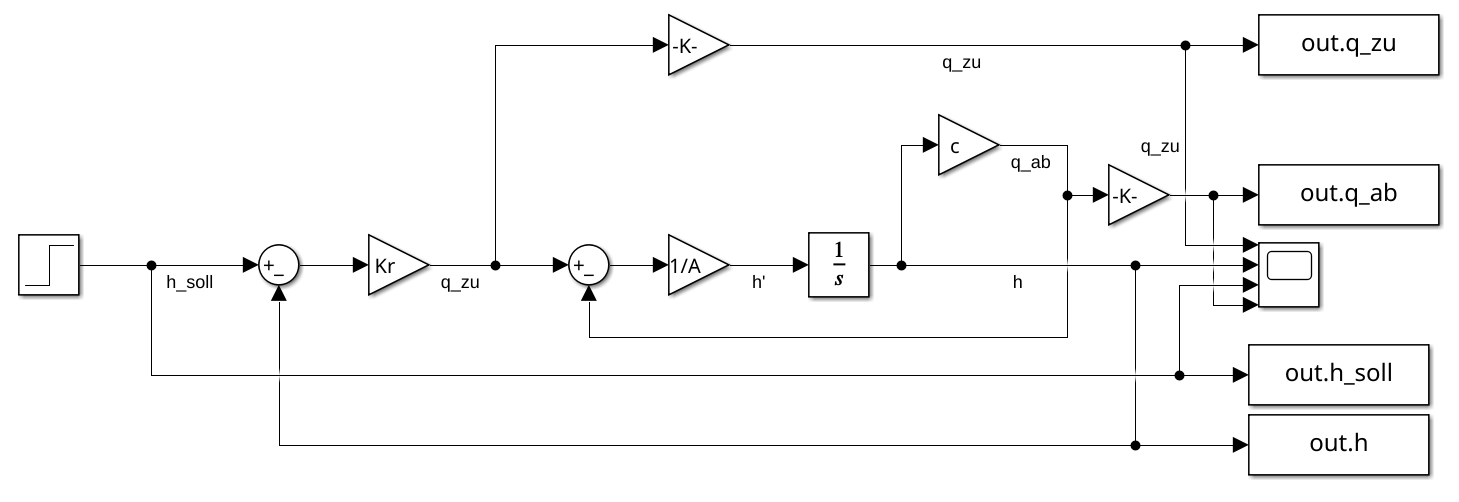
\includegraphics[width=0.9\textwidth]{graphix/a_modell_mit_abfluss.png}
    \caption{Blockschaltbild (Screenshot aus \textit{Simulink})}
    \label{blockschaltbild_a}
\end{figure}

\begin{figure}[p]
    \centering
    \begin{subfigure}{\textwidth}
    \centering
            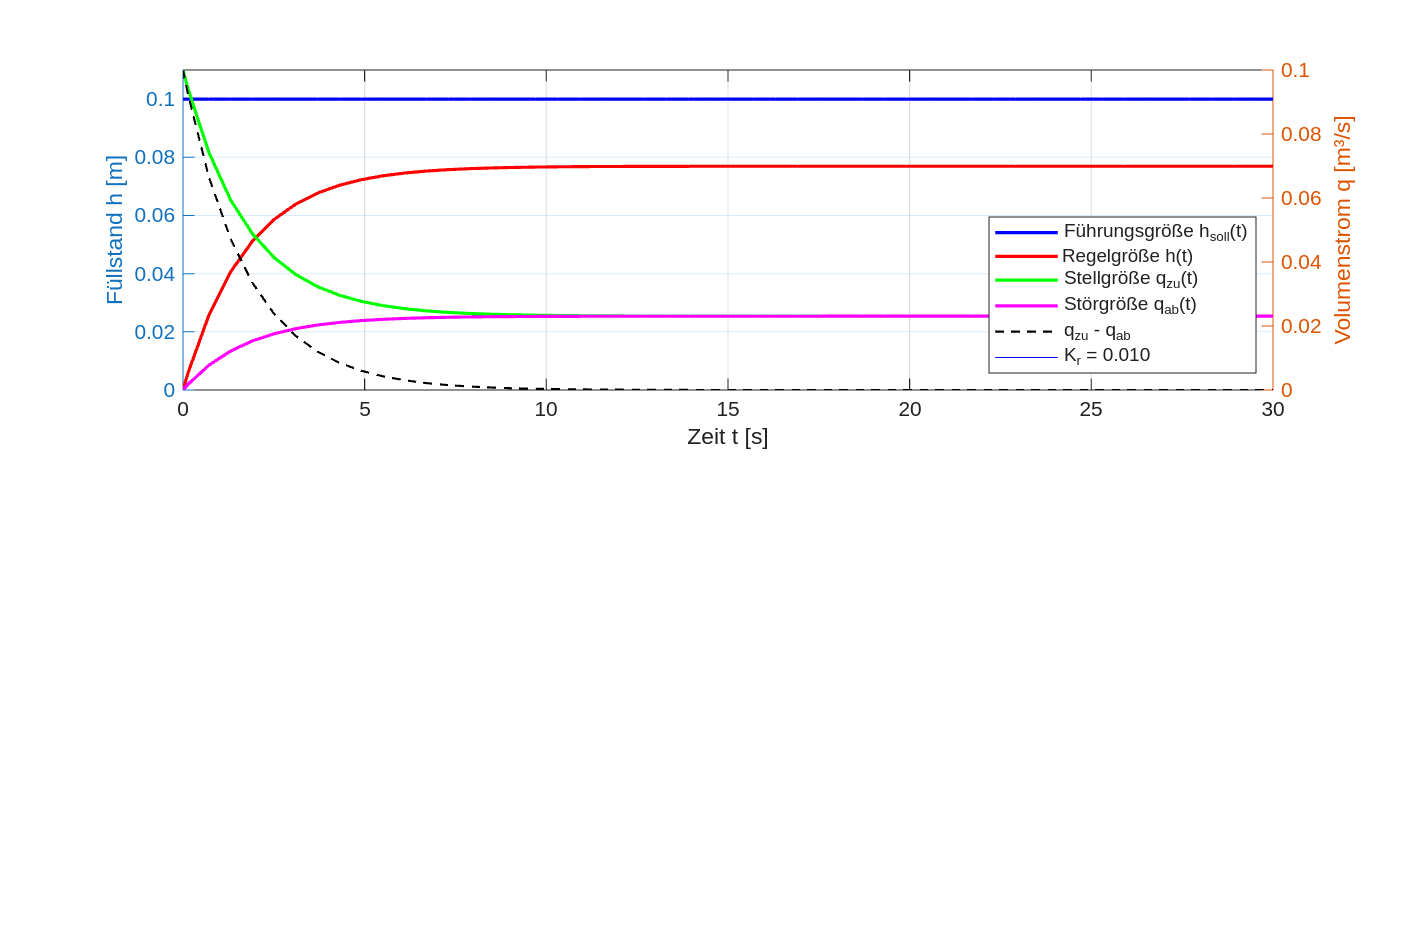
\includegraphics[trim=0cm 8cm 0cm 0.5cm, clip, width=0.9\textwidth]{graphix/a_modell_mit_abfluss_KR_0.0100.png}
    \end{subfigure}
    
    \begin{subfigure}{\textwidth}
        \centering
        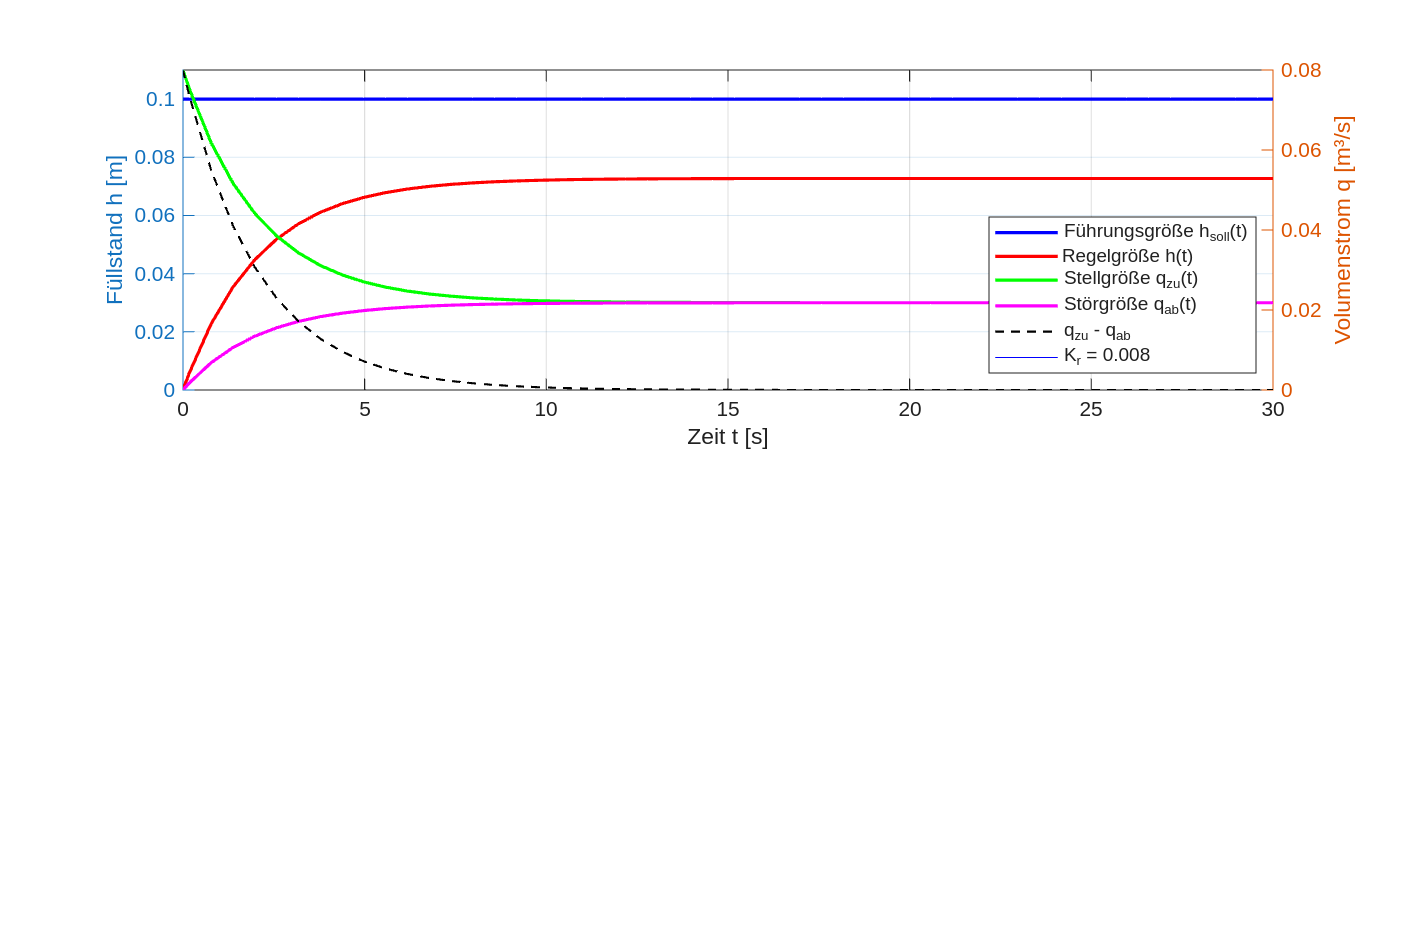
\includegraphics[trim=0cm 8cm 0cm 0.5cm, clip, width=0.9\textwidth]{graphix/a_modell_mit_abfluss_KR_0.0080.png}
    \end{subfigure}
    
    \begin{subfigure}{\textwidth}
        \centering
        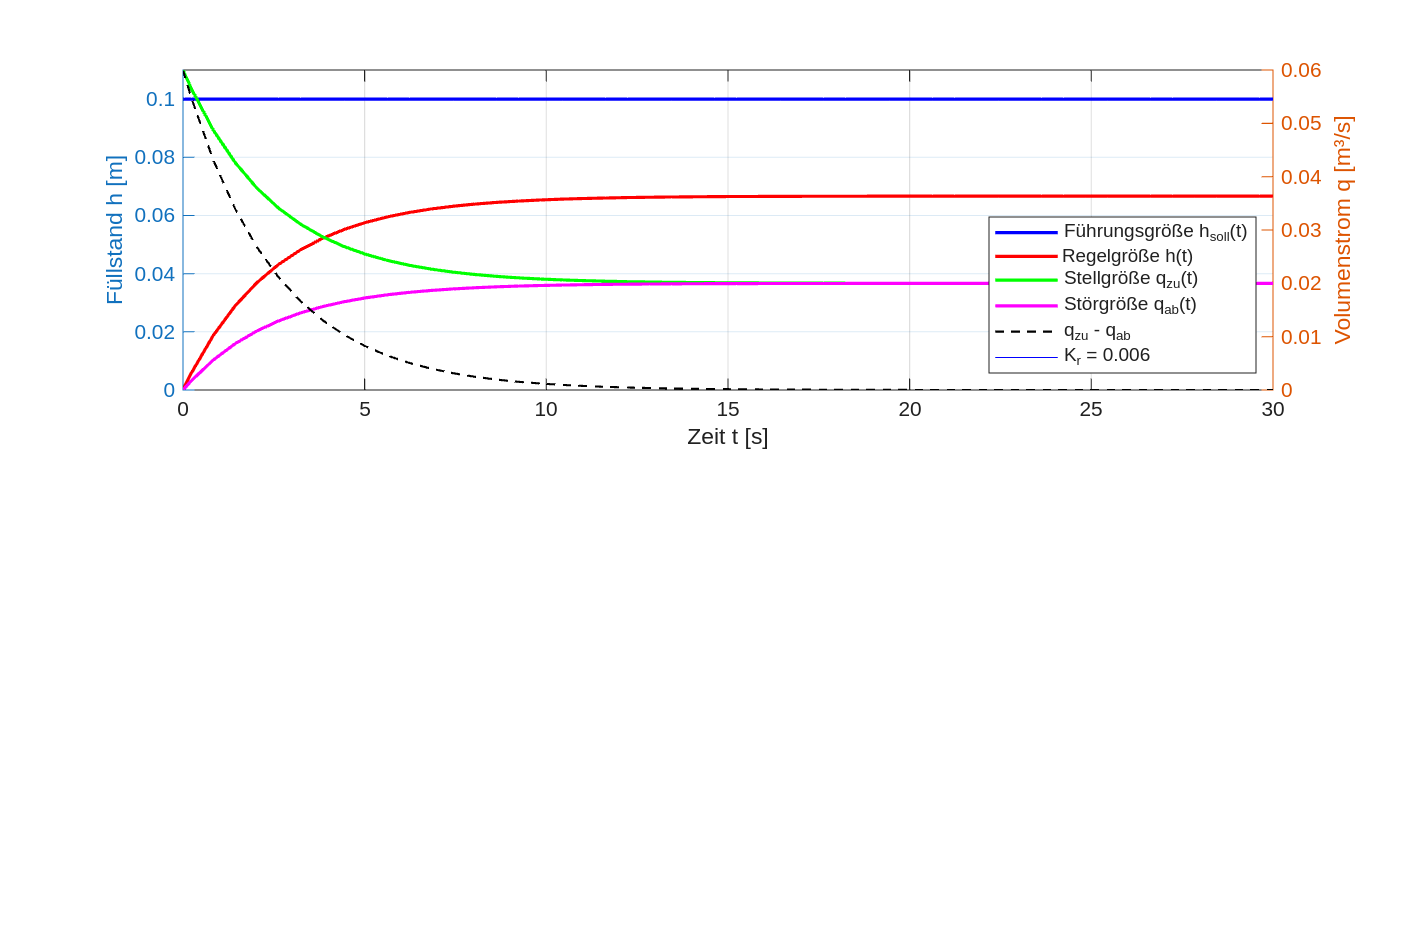
\includegraphics[trim=0cm 8cm 0cm 0.5cm, clip, width=0.9\textwidth]{graphix/a_modell_mit_abfluss_KR_0.0060.png}
    \end{subfigure}
    
    \begin{subfigure}{\textwidth}
        \centering
        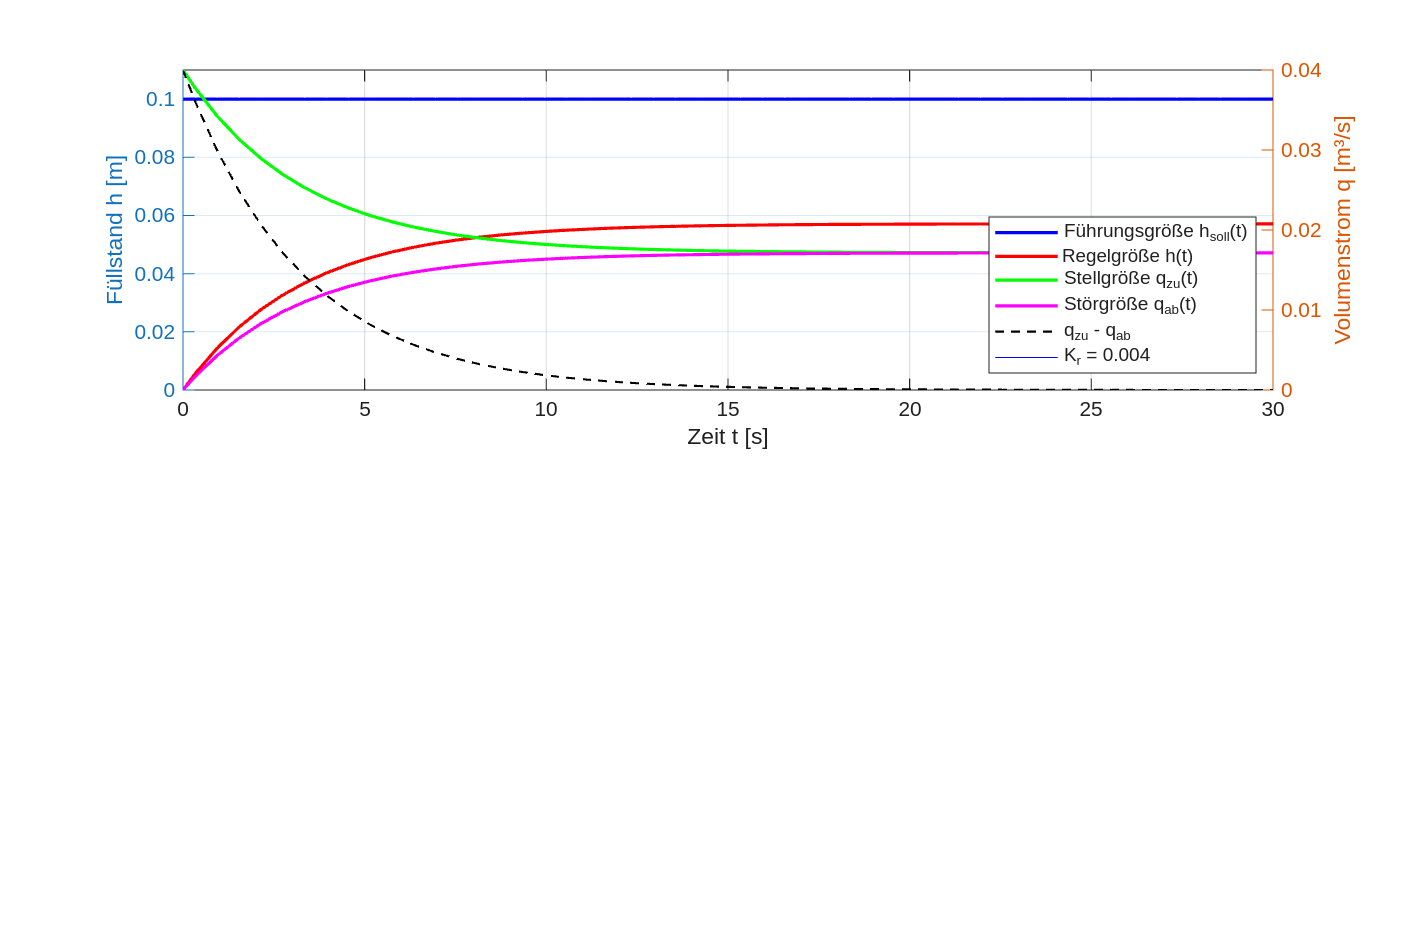
\includegraphics[trim=0cm 8cm 0cm 0.5cm, clip, width=0.9\textwidth]{graphix/a_modell_mit_abfluss_KR_0.0040.png}
    \end{subfigure}
    
    \begin{subfigure}{\textwidth}
        \centering
        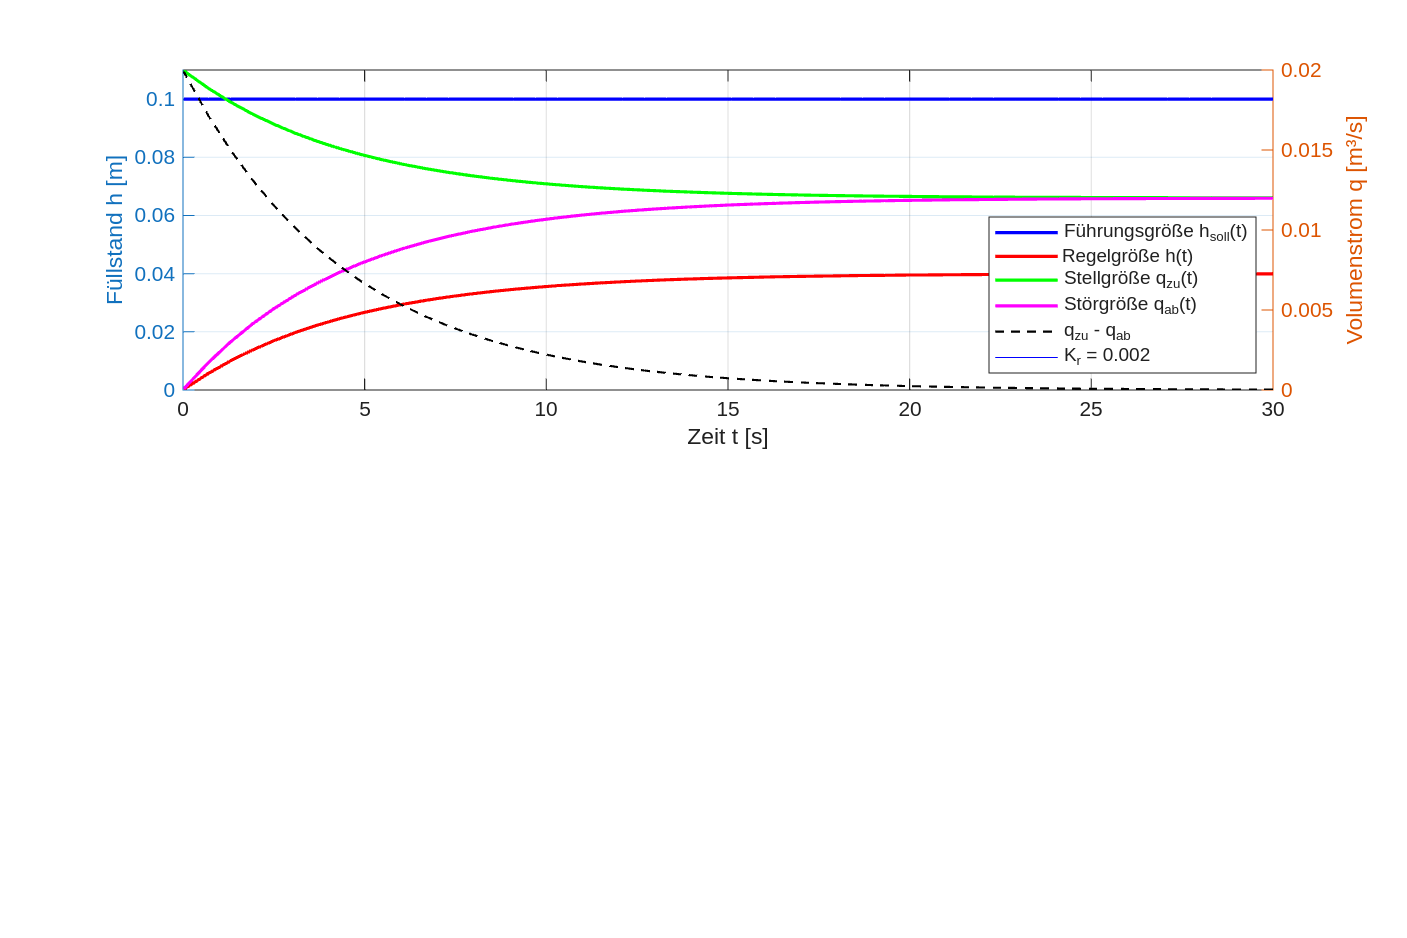
\includegraphics[trim=0cm 8cm 0cm 0.5cm, clip, width=0.9\textwidth]{graphix/a_modell_mit_abfluss_KR_0.0020.png}
    \end{subfigure}
    
    \caption{\textit{Matlab}-Plots für verschiedene Reglerverstärkungen}
    \label{fig:a_plots_mit_abfluss}
\end{figure}

\begin{figure}[H]
    \centering
    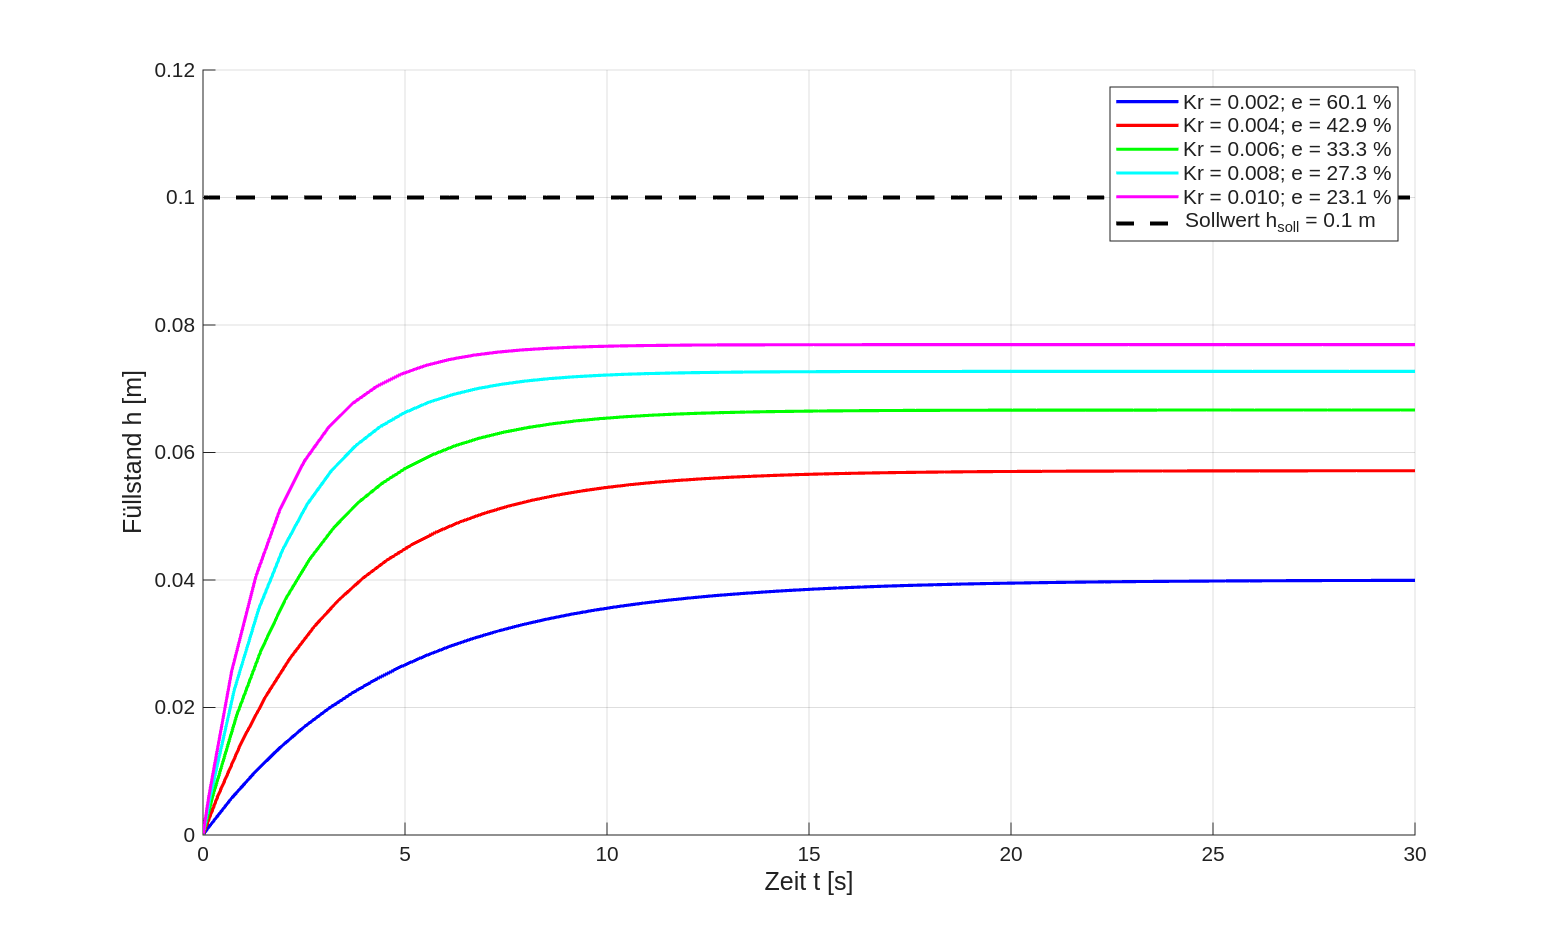
\includegraphics[width=0.9\textwidth]{graphix/a_modell_mit_abfluss_vergleich.png}
    \caption{Vergleich der stationären Endwerte}
    \label{vergleich_a}
\end{figure}

\begin{table}[h]
    \centering
    \caption{Reglerverstärkungen und Regelabweichungen}
    \label{tab:reglerparameter}
        \begin{tabularx}{\textwidth}{|>{\centering\arraybackslash}X|>
        {\centering\arraybackslash}X|>{\centering\arraybackslash}X|>{\centering\arraybackslash}X|}
        \hline
        Reglerverstärkung & Stationärer Endwert & Absolute Regelabweichung & Relative Regelabweichung \\
        $K_r$  & $h(t \to \infty)$ [m]& $e_{\text{abs}}$ [m]& $e_{\text{rel}}$ [\%] \\
        \hline

        0.010 & 0.0766 & 0.0234 & 23.39 \\
        \hline
        0.008 & 0.0720 & 0.0280 & 27.96 \\
        \hline
        0.006 & 0.0651 & 0.0349 & 34.87 \\
        \hline
        0.004 & 0.0541 & 0.0459 & 45.87 \\
        \hline
        0.002 & 0.0352 & 0.0648 & 64.82 \\
        \hline           
    \end{tabularx}
\end{table}

\newpage

\subsection{Linearisiertes Ausflussgesetz mit PI-Regler}
Ein besseres Modell erhält man, indem das Proportional-Glied $K_r$ des Regelkreises um einen integrativen Anteil erweitert wird. Aus dem P-Regler wird so ein PI-Regler. Das Verhalten eines PI-Reglers wird durch Gleichung (7) beschrieben.

\begin{equation}
    u(t)=K_r \cdot \left( e(t) + \frac{1}{T_n} \int e(t) \, dt \right)
\end{equation}

Zusätzlich zu der Reglerverstärkung $K_r$ muss nun auch die Nachstellzeit $T_n$ berücksichtig werden. In \textit{Simulink} wird ein PID-Regler ausgewählt und als PI-Regler definiert. Die Regelparameter werden nach Gleichung (8) festgelegt.

\begin{equation}
    P=K_r \quad \text{und} \quad I=\frac{1}{T_n}
\end{equation}

Für diese Simulation wird die Nachstellzeit variiert. Für die Reglerverstärkung wird $K_r=0.006$ ausgewählt. Für große Nachstellzeiten gibt es keine Überschwinger. Je kleiner die Nachstellzeit ist, desto mehr wird der integrale Anteil bezogen auf den proportionalen Anteil gewichtet und die Überschwinger nehmen zu. Gesucht ist die Nachstellzeit, für die es keine Überschwinger mehr gibt. Das Intervall wird in \textit{Matlab} iterativ gesucht. Als Erstes werden Nachstellzeiten zwischen \SI{100}{s} und \SI{0.01}{s} untersucht. Das Intervall wird immer kleiner gewählt, um einen möglichst exakten Wert für $T_n$ zu ermitteln. Für $T_n \geq$ \SI{6.2}{s} gibt es keine Überschwinger mehr.

Der \textit{Matlab}-Code ist in \ref{code_2b1} und \ref{code_2b2}. Abbildung \ref{blockschaltbild_b} zeigt das Modell. In der Abbildung \ref{fig:b_plots_mit_abfluss} sind die zeitlichen Verläufe der Signale für verschiedene Nachstellzeiten in dem exakten Intervall dargestellt. Dieses Intervall wird mit den jeweiligen Überschwingern in Abbildung \ref{vergleich_b} gezeigt. Tabelle \ref{tab:uberschwinger} zeigt die Überschwinger für verschiedene Nachstellzeiten und die iterativen Intervalle für die Ermittelung von $T_n$. 

\begin{sourcecode}
    \caption{\textit{Matlab}-Code zur Simulation und Berechnung der Überschwinger}
    \begin{minted}{matlab}
        assignin('base', 'A', A);
        assignin('base', 'c', c);
        assignin('base', 'Kr', Kr_fixed);

        %% Nachstellzeiten  
        %Tn_vector = [100, 50, 20, 10, 5, 2, 1, 0.5, 0.2, 0.1, 0.05, 0.02, 0.01];
        Tn_vector = [6.2, 6.15, 6.1, 6.05, 6];
        n_sim = length(Tn_vector);

        % Initialisierung 
        overshoot_percent = zeros(1, n_sim);
        has_overshoot = zeros(1, n_sim);
        steady_state_h = zeros(1, n_sim);
        max_h_values = zeros(1, n_sim);

        %% Simulationsparameter 
        run_time = 30;
        open_system('b_modell_mit_abfluss');
        set_param('b_modell_mit_abfluss', 'StopTime', num2str(run_time));
        set_param('b_modell_mit_abfluss', 'StartTime', '0');
        set_param('b_modell_mit_abfluss/Integrator', 'InitialCondition', '0');

        % Step-Block
        set_param('b_modell_mit_abfluss/Step', 'Time', '0');
        set_param('b_modell_mit_abfluss/Step', 'Before', '0');
        set_param('b_modell_mit_abfluss/Step', 'After', num2str(h_soll_wert));

        for i = 1:n_sim
            Tn = Tn_vector(i);
            Ki = 1/Tn; 
                       
            set_param('b_modell_mit_abfluss/PID Controller', 'P', num2str(Kr_fixed));
            set_param('b_modell_mit_abfluss/PID Controller', 'I', num2str(Ki));
            set_param('b_modell_mit_abfluss/PID Controller', 'D', '0');
            
            simOut = sim("b_modell_mit_abfluss.slx");
            
            if isstruct(simOut)
                t = simOut.tout;
                h = simOut.h;
                q_zu = simOut.q_zu;
                q_ab = simOut.q_ab;
                h_soll = simOut.h_soll;
            else
                t = simOut.get('tout');
                h = simOut.get('h');
                q_zu = simOut.get('q_zu');
                q_ab = simOut.get('q_ab');
                h_soll = simOut.get('h_soll');
            end
            
            if isa(h, 'timeseries')
                h = h.Data;
                t = t.Data;
                q_zu = q_zu.Data;
                q_ab = q_ab.Data;
            end
                                         
    \end{minted}
\label{code_2b1}
\end{sourcecode}

\begin{sourcecode}
    \caption{\textit{Matlab}-Code zur Simulation und Berechnung der Überschwinger}
    \begin{minted}{matlab}
        
            % Stationärer Endwert
            n_end = round(0.9 * length(h));
            h_end = mean(h(n_end:end));
            steady_state_h(i) = h_end;
            
            % Maximalen Wert finden
            idx_start = find(t > 2, 1, 'first');
            if isempty(idx_start)
                idx_start = 1;
            end
            h_max = max(h(idx_start:end));
            max_h_values(i) = h_max;
            
            % Überschwinger  
            if h_max > h_end * 1.01
                overshoot_percent(i) = (h_max - h_end) / h_end * 100;
                has_overshoot(i) = 1;
                fprintf('  -> ÜBERSCHWINGER: %.2f%% (h_max = %.4f m, h_end = %.4f m)\n'
                , ...
                        overshoot_percent(i), h_max, h_end);
            else
                overshoot_percent(i) = 0;
                has_overshoot(i) = 0;
                fprintf('  -> Kein Überschwinger (h_max = %.4f m, h_end = %.4f m)\n', 
                h_max, h_end);
            end

    ... 

            % Intervallbestimmung
            Tn_overshoot = Tn_vector(has_overshoot == 1);
            Tn_no_overshoot = Tn_vector(has_overshoot == 0);

            if ~isempty(Tn_no_overshoot) && ~isempty(Tn_overshoot)
                Tn_max_no_overshoot = max(Tn_no_overshoot);    
                Tn_min_overshoot = min(Tn_overshoot);          
                
                fprintf('  Keine Überschwinger für TN ≥ %.4f s\n', 
                Tn_max_no_overshoot);
                fprintf('  Überschwinger vorhanden für TN ≤ %.4f s\n', Tn_min_overshoot);
                fprintf('  Grenzbereich: %.4f s < TN_kritisch < %.4f s\n', 
                Tn_max_no_overshoot, Tn_min_overshoot);
                
            elseif isempty(Tn_no_overshoot)
                fprintf('  Bei allen getesteten TN-Werten treten Überschwinger auf!\n');
            elseif isempty(Tn_overshoot)
                fprintf('  Bei keinem getesteten TN-Wert treten Überschwinger auf!\n');
            end                                     
    \end{minted}
\label{code_2b2}
\end{sourcecode}

\begin{figure}[H]
    \centering
    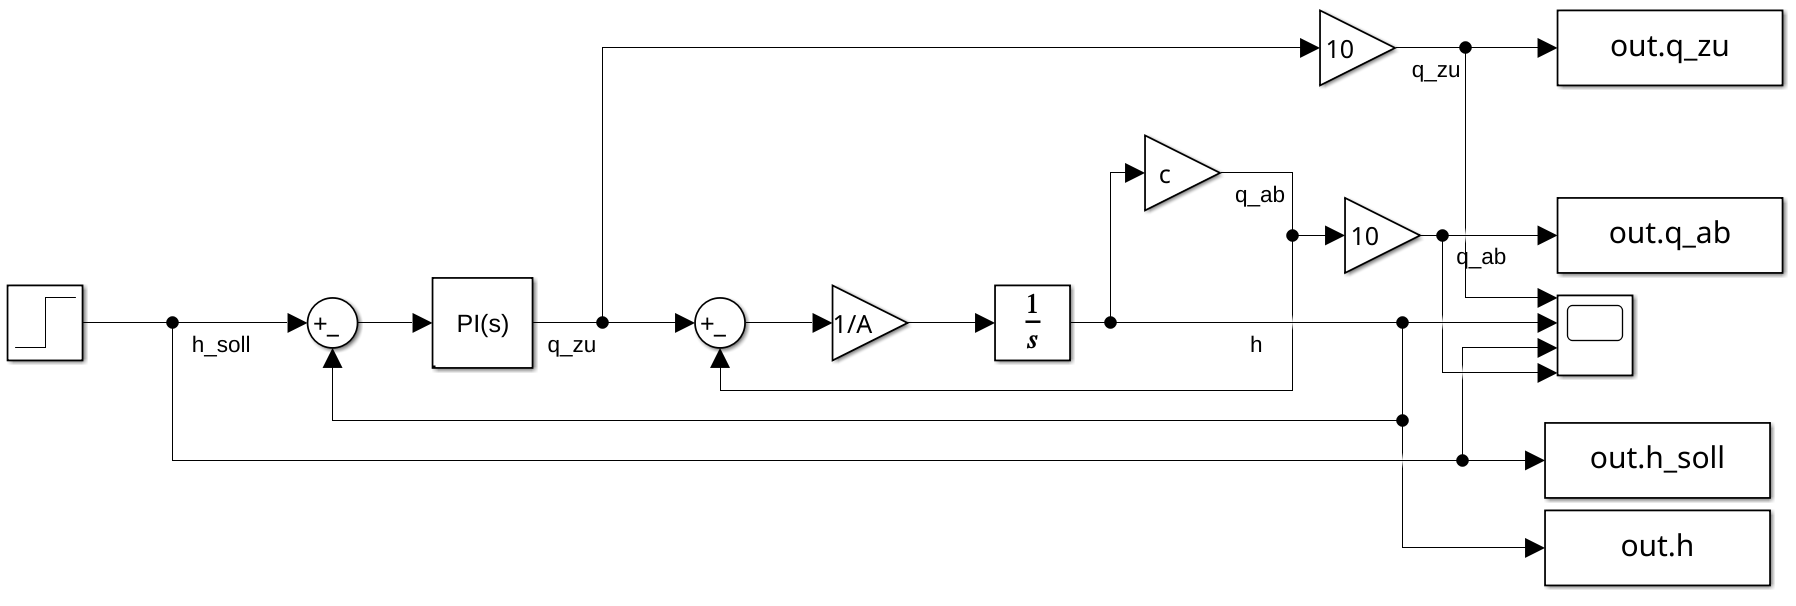
\includegraphics[width=0.9\textwidth]{graphix/b_modell_mit_abfluss.png}
    \caption{Blockschaltbild (Screenshot aus \textit{Simulink})}
    \label{blockschaltbild_b}
\end{figure}

\begin{figure}[p]
    \centering
    \begin{subfigure}{\textwidth}
    \centering
            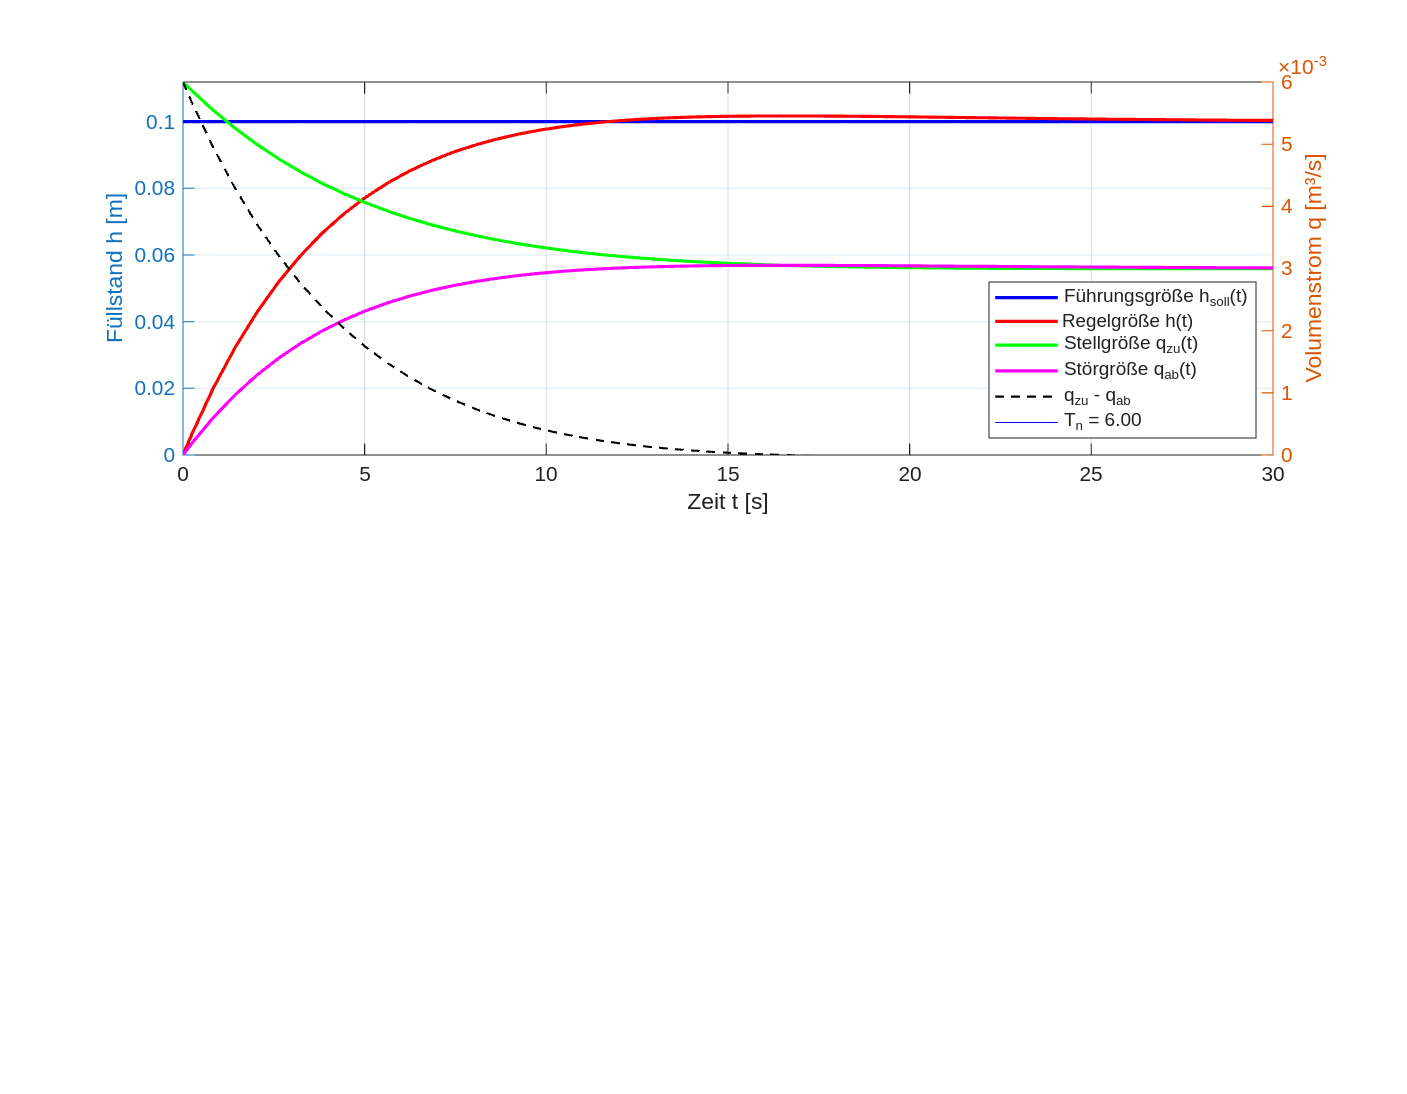
\includegraphics[trim=0cm 9.5cm 0cm 0.5cm, clip, width=0.9\textwidth]{graphix/b_modell_mit_abfluss_TN_6.00.png}
    \end{subfigure}
    
    \begin{subfigure}{\textwidth}
        \centering
        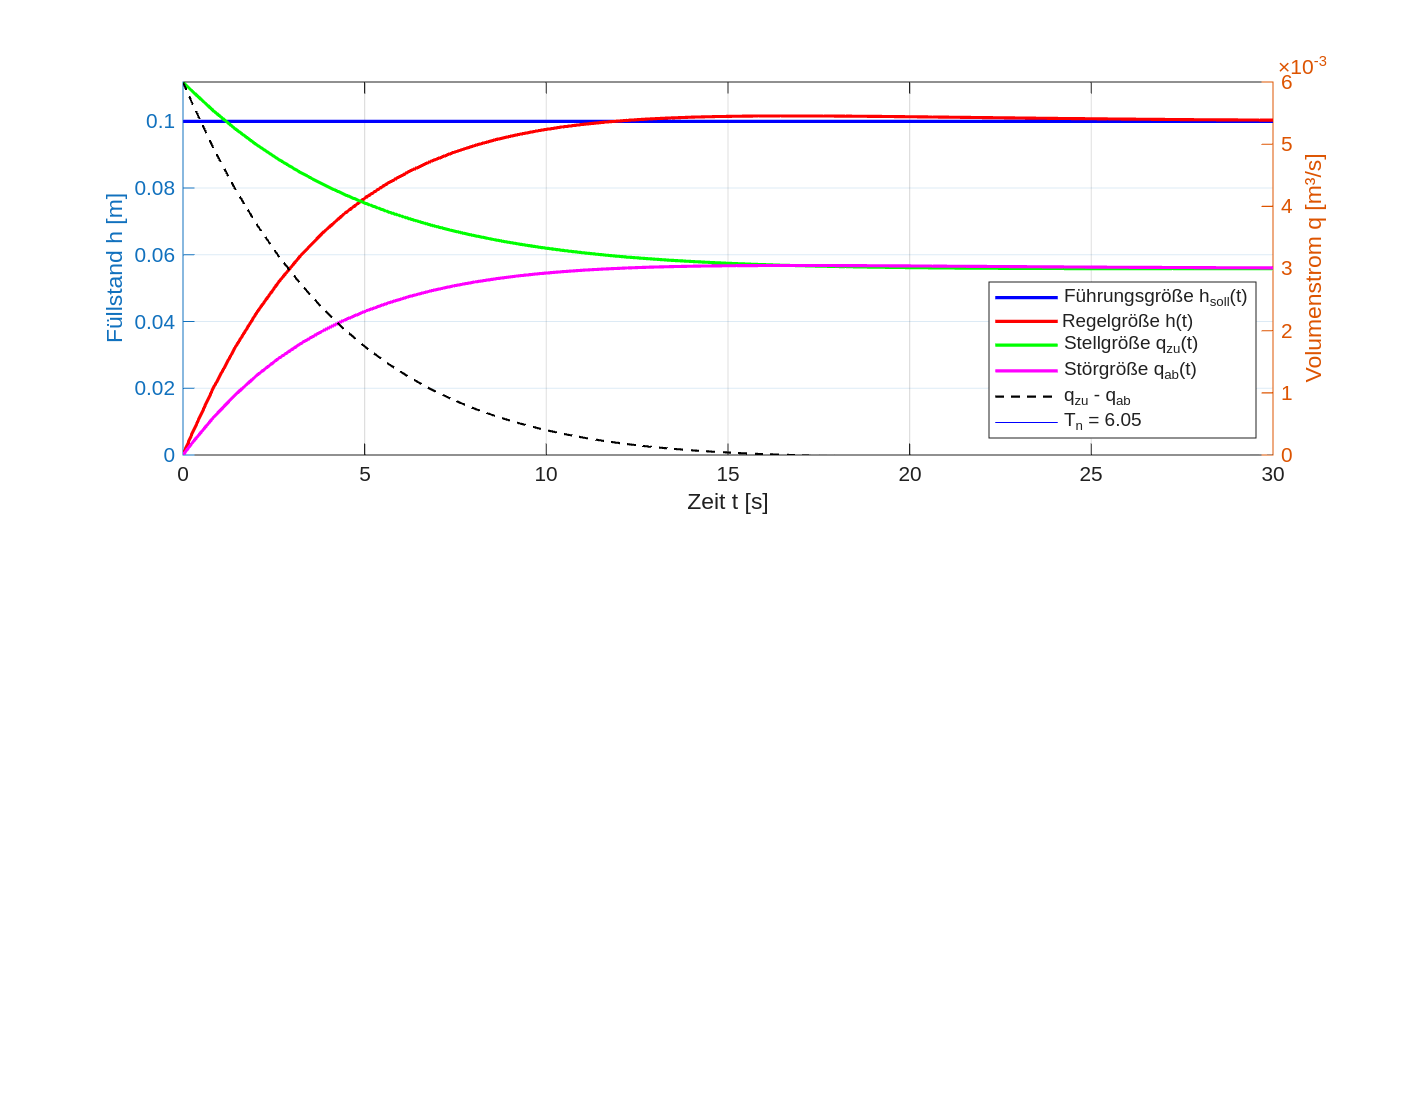
\includegraphics[trim=0cm 9.5cm 0cm 0.5cm, clip, width=0.9\textwidth]{graphix/b_modell_mit_abfluss_TN_6.05.png}
    \end{subfigure}
    
    \begin{subfigure}{\textwidth}
        \centering
        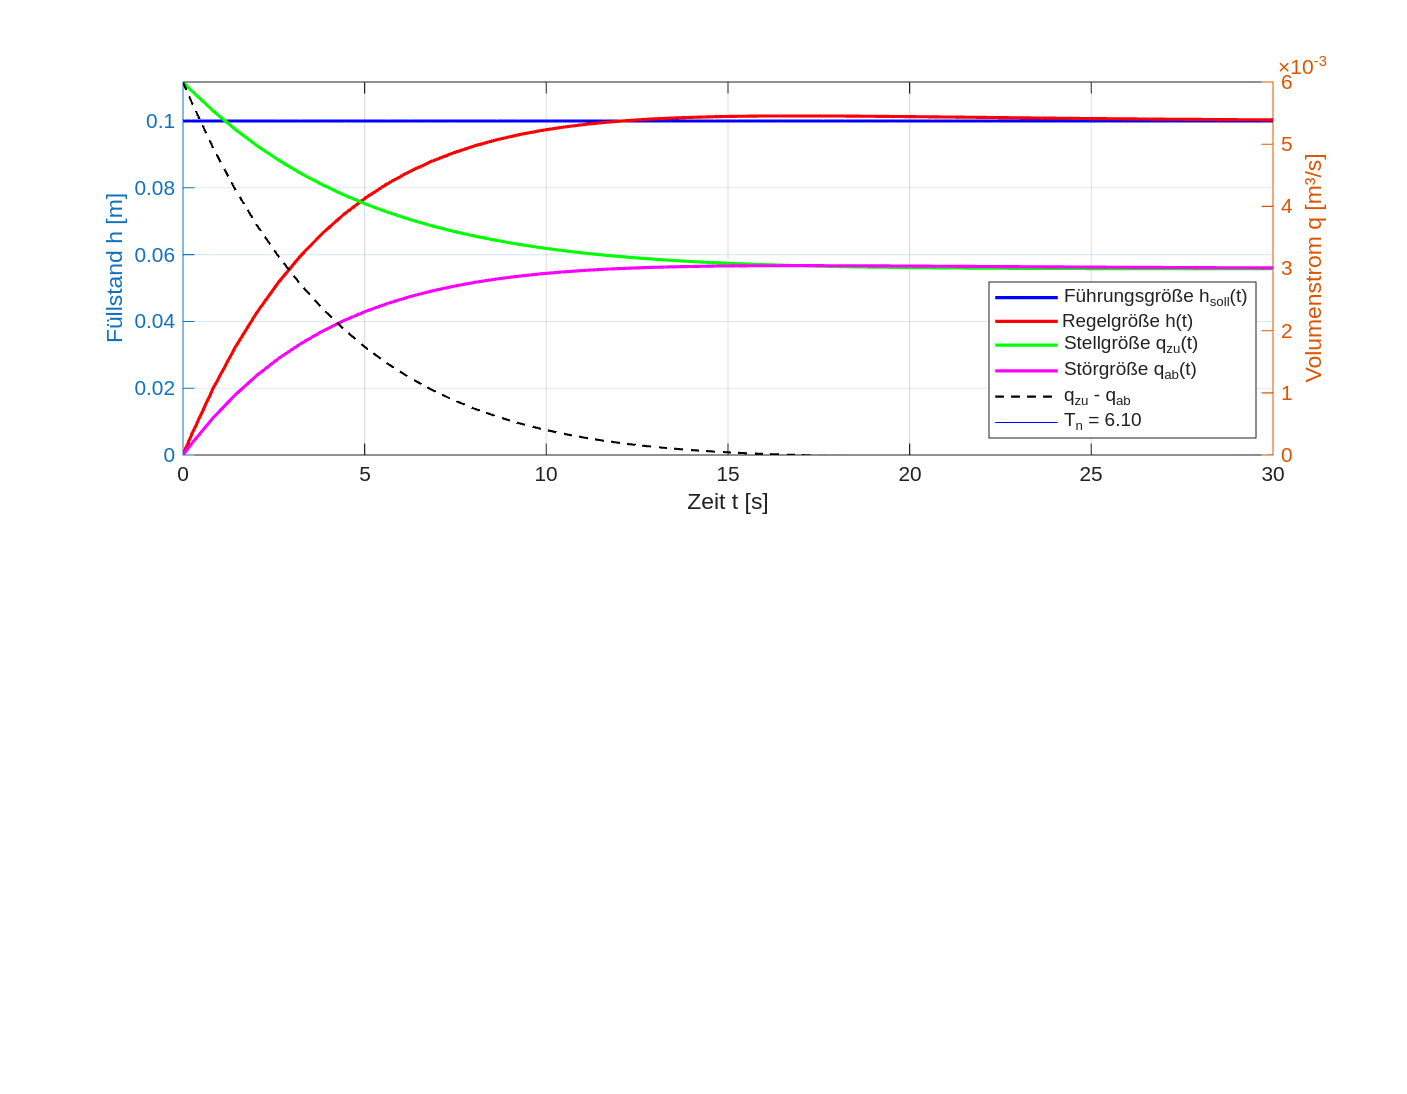
\includegraphics[trim=0cm 9.5cm 0cm 0.5cm, clip, width=0.9\textwidth]{graphix/b_modell_mit_abfluss_TN_6.10.png}
    \end{subfigure}
    
    \begin{subfigure}{\textwidth}
        \centering
        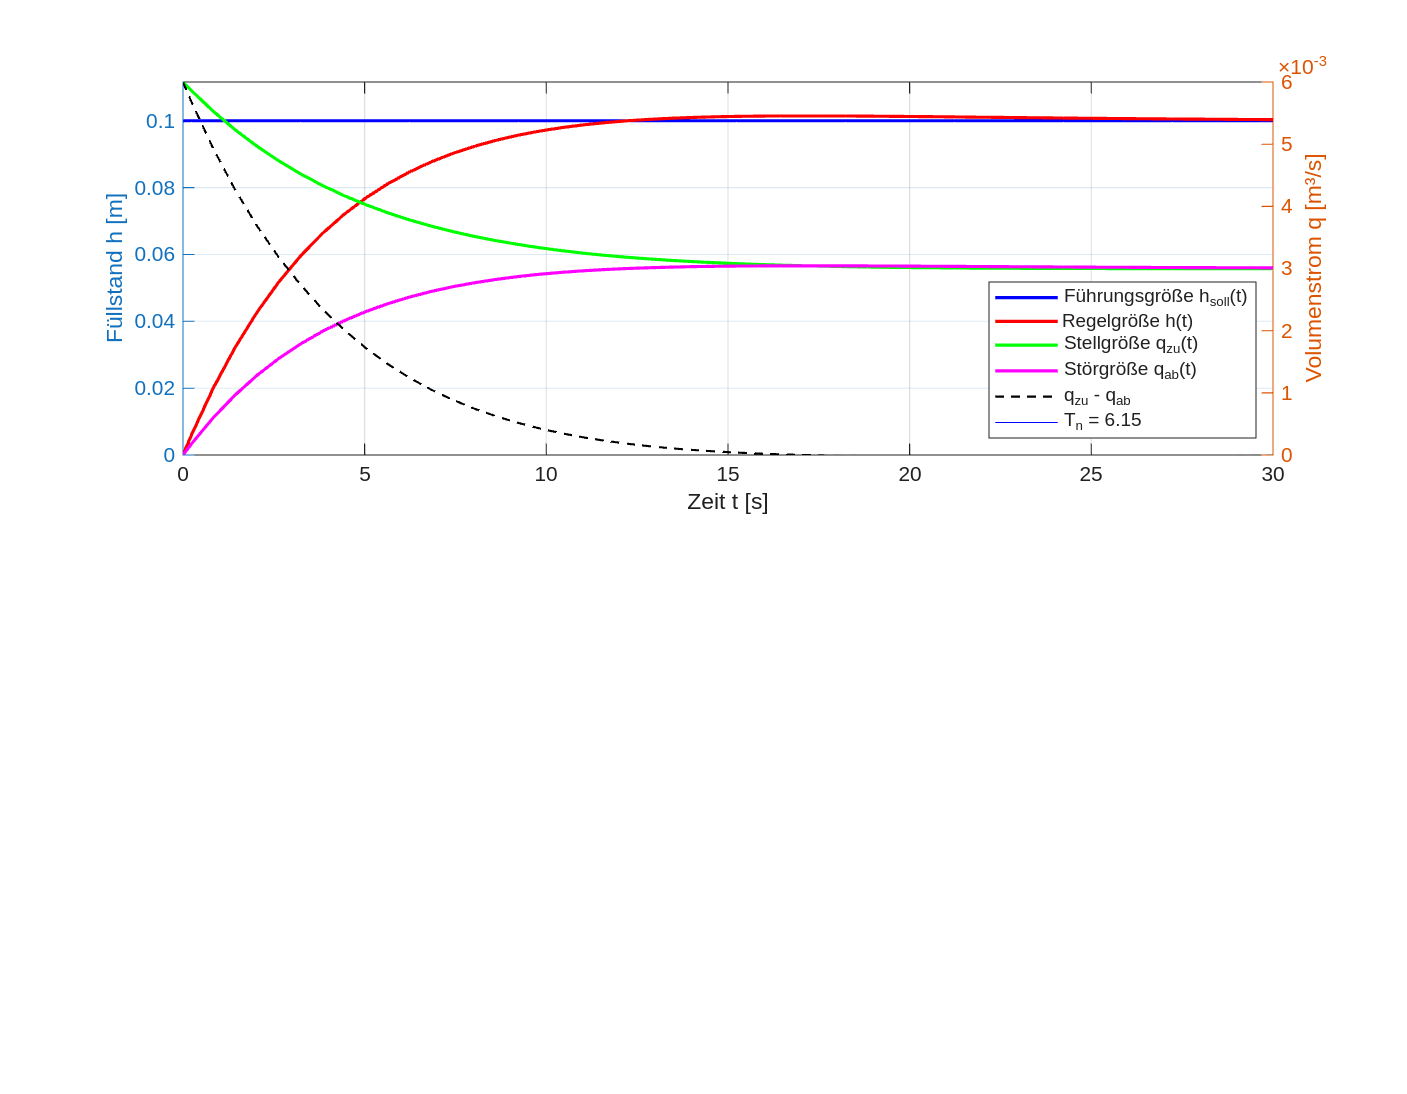
\includegraphics[trim=0cm 9.5cm 0cm 0.5cm, clip, width=0.9\textwidth]{graphix/b_modell_mit_abfluss_TN_6.15.png}
    \end{subfigure}
    
    \begin{subfigure}{\textwidth}
        \centering
        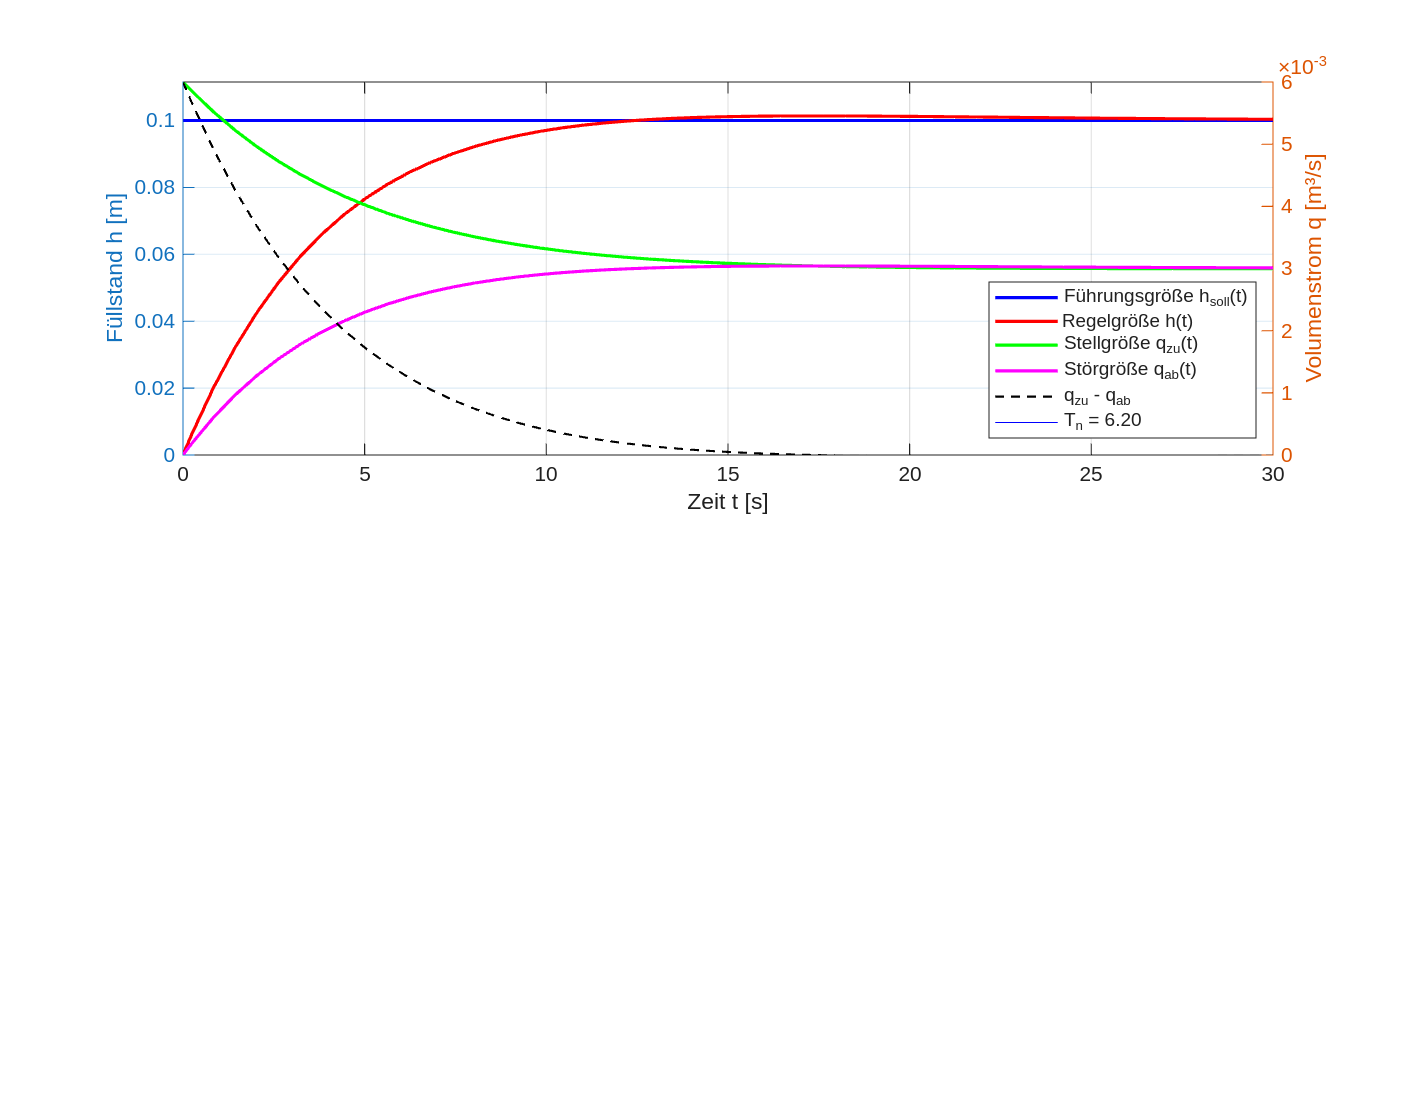
\includegraphics[trim=0cm 9.5cm 0cm 1cm, clip, width=0.9\textwidth]{graphix/b_modell_mit_abfluss_TN_6.20.png}
    \end{subfigure}
    
    \caption{\textit{Matlab}-Plots für verschiedene Rückstellzeiten}
    \label{fig:b_plots_mit_abfluss}
\end{figure}

\begin{figure}[H]
    \centering
    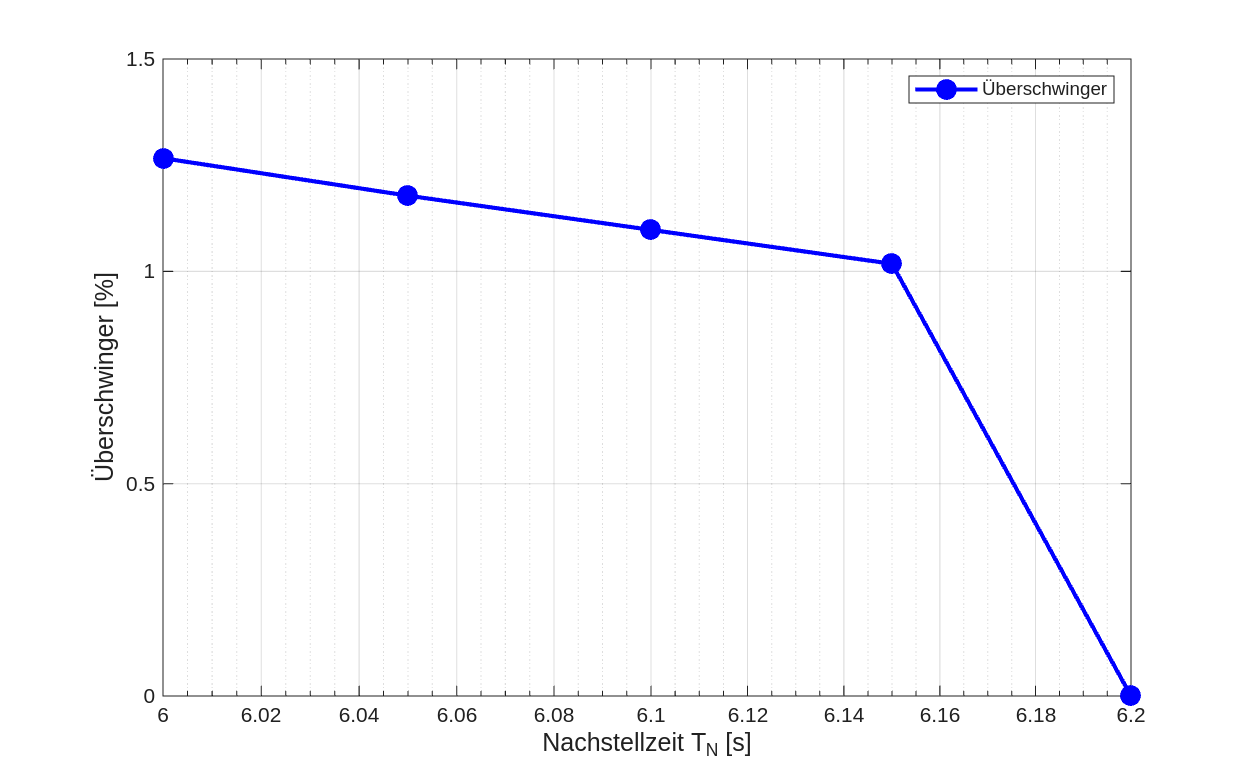
\includegraphics[width=0.9\textwidth]{graphix/b_modell_mit_abfluss_uberschwinger.png}
    \caption{Vergleich der Überschwinger}
    \label{vergleich_b}
\end{figure}


\begin{table}[h]
    \centering
    \caption{Reglerverstärkungen und Regelabweichungen}
    \label{tab:uberschwinger}
        \begin{tabularx}{\textwidth}{|>{\centering\arraybackslash}X|>
        {\centering\arraybackslash}X|}
        \hline
        Rückstellzeit & Überschwinger \\
        $T_n$ [s] & [\%] \\
        \hline
        100 & 0.00 \\ \hline
        50 & 0.00 \\ \hline
        20 & 0.00 \\ \hline
        10 & 0.00 \\ \hline
        9 & 0.00 \\ \hline
        8 & 0.00 \\ \hline
        7 & 0.00 \\ \hline
        6.8 & 0.00 \\ \hline
        6.6 & 0.00 \\ \hline
        6.4 & 0.00 \\ \hline
        6.2 & 0.00 \\ \hline
        6 & 1.20 \\ \hline
        5 & 3.51 \\ \hline
        2 & 18.23 \\ \hline
        1 & 31.67 \\ \hline
        0.5 & 43.81 \\ \hline
        0.2 & 58.45 \\ \hline
        0.1 & 64.30 \\ \hline
        0.05 & 71.86 \\ \hline
        0.02 & 54.80 \\ \hline
        0.01 & 64.00 \\ \hline
    \end{tabularx}
\end{table}

\newpage

\subsection{Ausflussgesetz nach Torricelli}
Eine physikalisch exakte Beschreibung des Ausflussverhaltens von Wasser liefert der Satz von Torricelli. Demnach hängt die Ausflussgeschwindigkeit und damit der Abfluss nur vom Füllstand ab. Der mathematische Zusammenhang ist in Gleichung (9) dargestellt. Es wird gefordert, dass sich bei einem Füllstand von $h=$ \SI{5}{cm} ein Abfluss von $q_{ab}=$ \SI{0.3}{\frac{l}{s}} ergibt.

\begin{equation}
    q_{ab}(t)=k\cdot \sqrt{h(t)} \quad \Longrightarrow \quad k=\frac{q_{ab}(t)}{\sqrt{h(t)}} = 0.0013416
\end{equation}

In Abbildung \ref{blockschaltbild_b} wird der Ausgang der Regelstrecke über den proportionalen Faktor $c$ rückgekoppelt. Dieser Faktor muss entsprechend des Satzes von Torricelli erweitert werden. Zuerst wird der Betrag des Signals gebildet, um negative Eingänge für den nachfolgenden Wurzelblock zu vermeiden. Danach wird das Signal um den Faktor $k$ verstärkt. Der Code für die Simulation ist in \ref{code_2c} zu finden. Das erweiterte Modell ist in Abbildung \ref{blockschaltbild_c} abgebildet. Die Simulation arbeitet mit den selben Werte für die Reglerverstärkung und die Nachstellzeit: $K_r=$ \SI{0.006}{} und $T_n=$ \SI{6.2}{s}. Der zeitliche Verlauf der Signale ist in Abbildung \ref{plot_c} abgebildet.

Der PI-Regler zeigt auch mit dem nichtlinearen Torricelli-Abflussgesetz eine sehr gute stationäre Genauigkeit. Der Füllstand erreicht einen stationären Endwert von $h(t \to \infty) = $ \SI{10.05}{cm}. Die Regelabweichung beträgt nur 0.48\%, was praktisch einer exakten Regelung entspricht.
Im Vergleich zum linearen Abflussmodell zeigt das Torricelli-Modell ein verändertes Einschwingverhalten. Die nichtlineare Kennlinie führt zu einer geringeren Dämpfung, was sich in einem größeren Überschwinger bemerkbar macht.
Mit den übernommenen Reglerparametern treten im Torricelli-Fall deutliche Überschwinger auf. Dies liegt daran, dass der nichtlineare Abfluss bei niedrigem Füllstand geringer ist als im linearen Modell, wodurch der Regler zunächst zu stark regelt.

\begin{sourcecode}
    \caption{\textit{Matlab}-Code zur Simulation mit dem Torricelli-Ausflussgesetz}
    \begin{minted}{matlab}
            assignin('base', 'k', k);
            assignin('base', 'A', A);
            assignin('base', 'Kr', Kr_fixed);
            assignin('base', 'Ki', Ki);
            assignin('base', 'h_soll_wert', h_soll_wert);

            %% Simulationsparameter 
            run_time = 30;
            open_system('c_modell_mit_abfluss');
            set_param('c_modell_mit_abfluss', 'StopTime', 'run_time');
            set_param('c_modell_mit_abfluss', 'StartTime', '0');

            % Step-Block 
            set_param('c_modell_mit_abfluss/Step', 'Time', '0');
            set_param('c_modell_mit_abfluss/Step', 'Before', '0');
            set_param('c_modell_mit_abfluss/Step', 'After', num2str(h_soll_wert));

            simOut = sim("c_modell_mit_abfluss.slx");

            %% Daten auslesen 
            if isstruct(simOut)
                t = simOut.tout;
                h = simOut.h;
                q_zu = simOut.q_zu;
                q_ab = simOut.q_ab;
                h_soll = simOut.h_soll;
            else
                t = simOut.get('tout');
                h = simOut.get('h');
                q_zu = simOut.get('q_zu');
                q_ab = simOut.get('q_ab');
                h_soll = simOut.get('h_soll');
            end

            % Bei timeseries-Objekten: Daten extrahieren
            if isa(h, 'timeseries')
                h = h.Data;
                t = t.Data;
                q_zu = q_zu.Data;
                q_ab = q_ab.Data;
                h_soll = h_soll.Data;
            end

            %% Stationärer Endwert 
            n_end = round(0.9 * length(h));
            h_end = mean(h(n_end:end));
            q_ab_end = mean(q_ab(n_end:end));
            q_zu_end = mean(q_zu(n_end:end));

            fprintf('Stationäre Werte (letzte 10%%):\n');
            fprintf('  h(∞) = %.4f m (%.1f cm)\n', h_end, h_end*100);
            fprintf('  q_ab(∞) = %.6f m³/s (%.3f L/s)\n', q_ab_end, q_ab_end*1000);
            fprintf('  q_zu(∞) = %.6f m³/s (%.3f L/s)\n', q_zu_end, q_zu_end*1000);                              
    \end{minted}
\label{code_2c}
\end{sourcecode}

\begin{figure}[H]
    \centering
    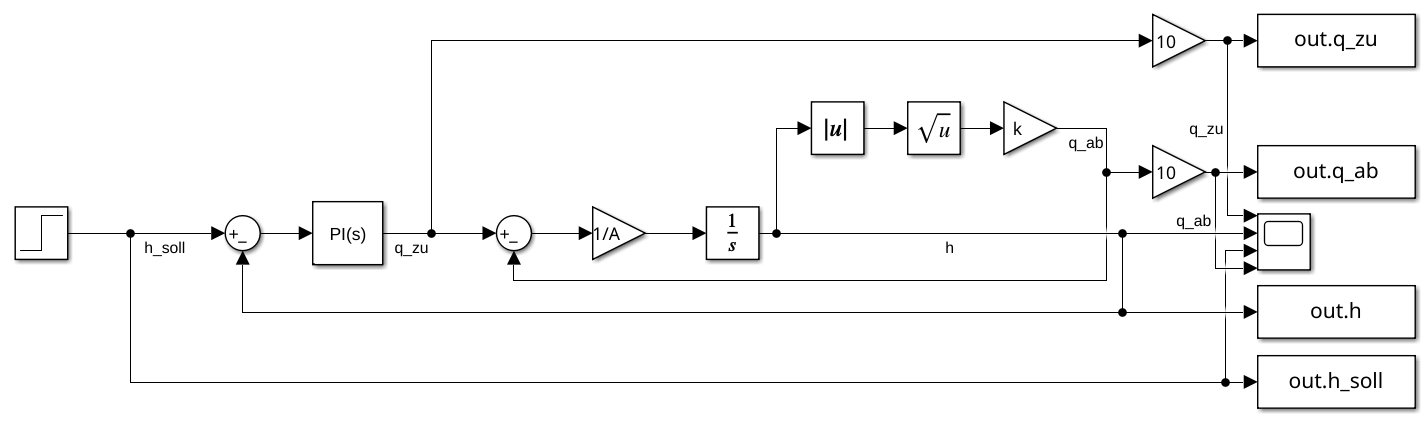
\includegraphics[width=0.9\textwidth]{graphix/c_modell_mit_abfluss.png}
    \caption{Blockschaltbild (Screenshot aus \textit{Simulink})}
    \label{blockschaltbild_c}
\end{figure}

\begin{figure}[H]
    \centering
    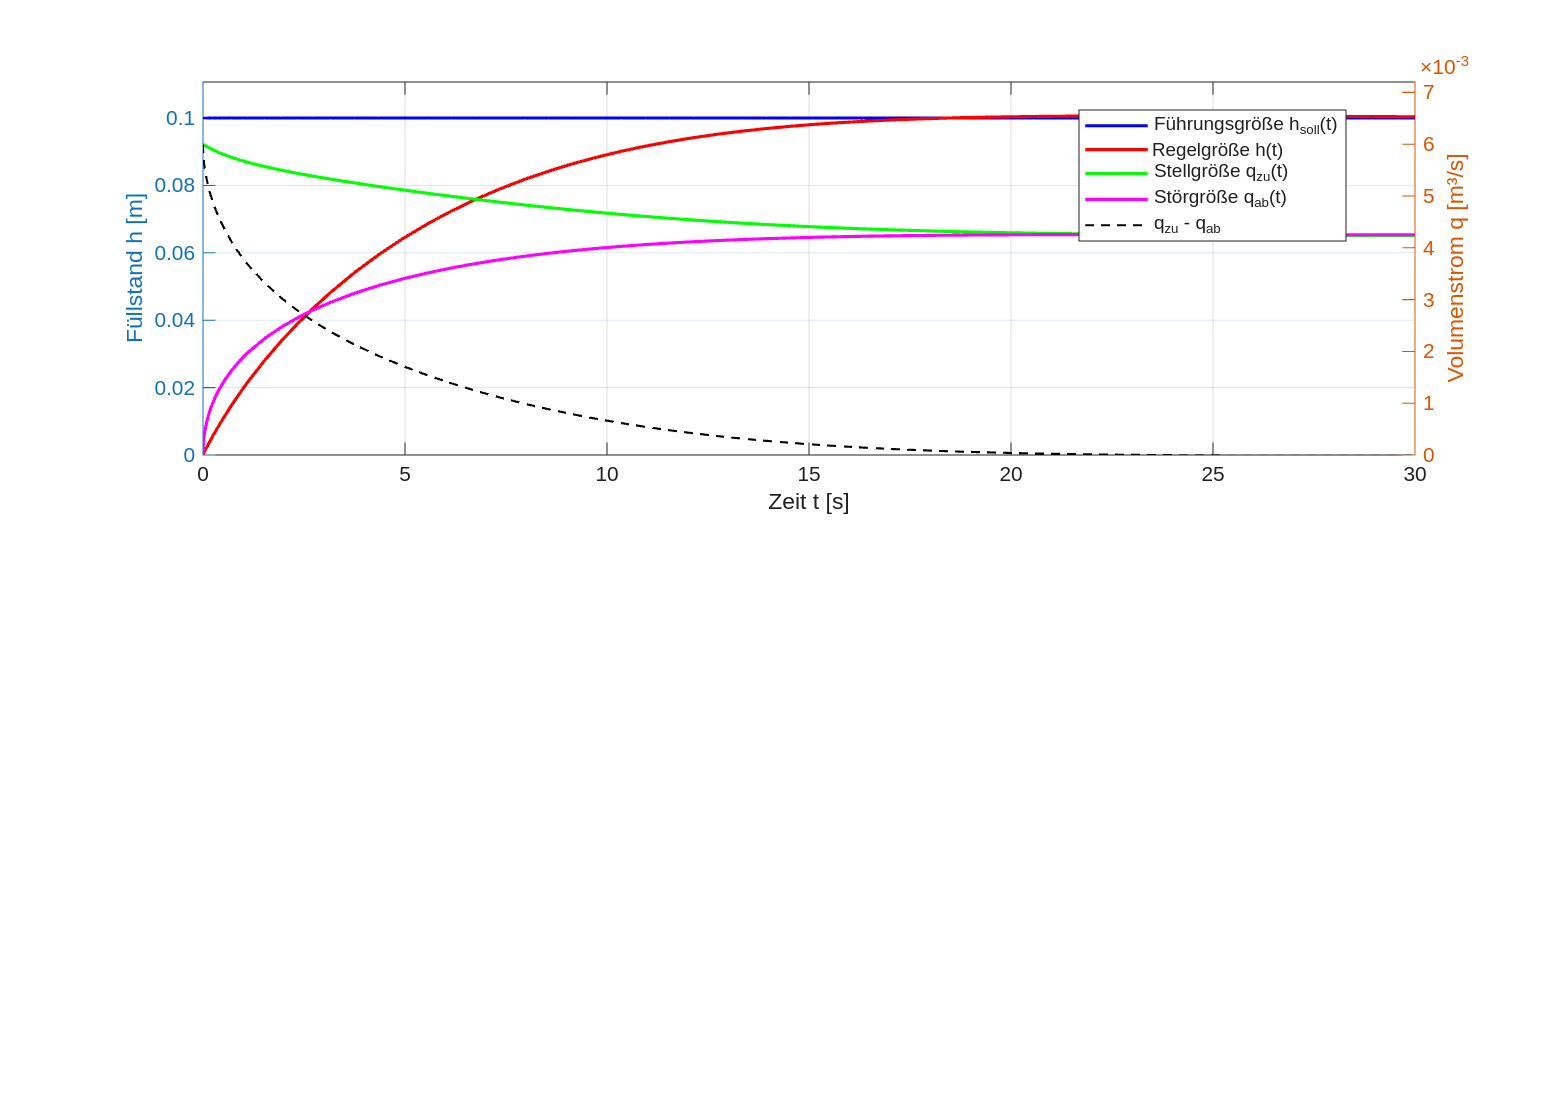
\includegraphics[trim=1.8cm 9.5cm 1.8cm 0.5cm, clip, width=\textwidth]{graphix/c_modell_mit_abfluss_torricelli.png}
    \caption{\textit{Matlab}-Plot für $K_r=0.006$ und $T_n=6.2s$}
    \label{plot_c}
\end{figure}
